\chapter{Illustrazione e Sviluppo}
\section{Hardware}
In questa sezione verranno presi in esame più specificatamente i componenti della plancia. Le caratteristiche tecniche del computer sono già state approfondite nell’apposito capitolo dedicato al restauro e non sono necessarie spiegazioni ulteriori. Ecco invece i pezzi che non sono ancora stati illustrati.
\subsection{Pulsanti}
I pulsanti usati per il progetto hanno una particolaritá molto interessante. I \textit{Chrome Effect Illuminated Arcade Button} (Figura~\ref{fig:button}) sono provvisti di led alimentabili a 12 Volt. Sul cabinato sono stati usati led di quattro colori diversi (blu, rosso, bianco, verde). I pulsanti sono costantemente alimentati quando la macchina all'interno del cabinet è in funzione. Non si illuminano solo alla pressione come i pulsanti di un DDR, sia per poca praticità della scelta sia per questioni estetiche. I pulsanti da soli sarebbero semplici pezzi di plastica inutili senza i Microswitch. La scelta di questi componenti tra la vasta gamma presente negli shop online non è stata affatto difficili da compiere. Esistono diversi tipi di Microswitch, le opzioni di acquisto erano incentrate principalmente su tre tipi: E-Switch, Chen Xiao e D44X Cherry. Anche se i primi due sarebbero stati molto più economici, non c’è stato alcun dubbio sulla scelta d’acquisto. I D44X Cherry sono i migliori Microswitch in commercio. Ad un prezzo poco più alto del normale, è garantita l’alta qualità del prodotto, un click gradevole e morbido e l’altissima durabilità nel tempo.\\I microswitch vanno inseriti nei bulb holder che a loro volta hanno un incastro nei bottini.\\
\begin{figure}[!ht]
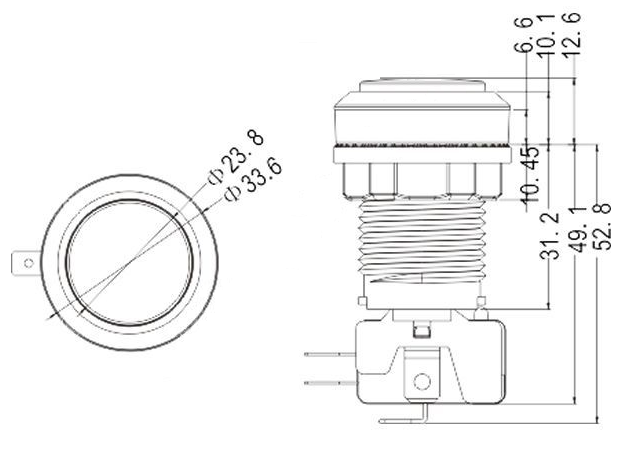
\includegraphics[scale=0.45]{button}
\centering
\caption{Chrome Effect Illuminated Arcade Button (misure in mm)}
\label{fig:button}
\end{figure}
\\I componenti di un pulsante intero sono:\\
\textbf{Button}: Il pulsante che viene premuto con la pressione delle dita.\\
\textbf{Fixing ring}: Un pezzo di plastica da stringere per fissare il bottone alla plancia.\\
\textbf{Spacer}: Un pezzo di plastica che può essere usato come eventuale spessore aggiuntivo.\\
\textbf{Bulb holder}: È il socket in cui va inserito il led. È paragonabile all’alloggiamento per lampadine di una lampada.\\
\textbf{Led}: Un diodo led va inserito nel Bulb holder di ogni singolo bottone.\\
\textbf{Microswitch}: Il piccolo interruttore che viene premuto alla pressione del bottone. È suo compito inviare segnali elettrici alla scheda di encoding.\\
\subsection{Joystick}
There are two types of joystick handles: Ball Top (that is spherical) and Bat Top (that is tear shaped). The two Joysticks used on the cabinet are Ball Top, manufactured by the japanese company Sanwa. The \textit{SANWA JLF-TP-8YT} (Figure~\ref{fig:joystick}) is one of the most popular products thanks to its precision and sensibility. That’s why it is considered one of the best picks by the expert players of fighting games, in which every millisecond is important. The joystick has a Restrictor Gate which allows to achieve eight different movements. There are just four microswitches, so pressing two of them contemporarily allows the user to move in eight directions. The connection to the keyboard encoder is simple and fast thanks to a five pin connector (one of them is the ground).\\
\begin{figure}[!h]
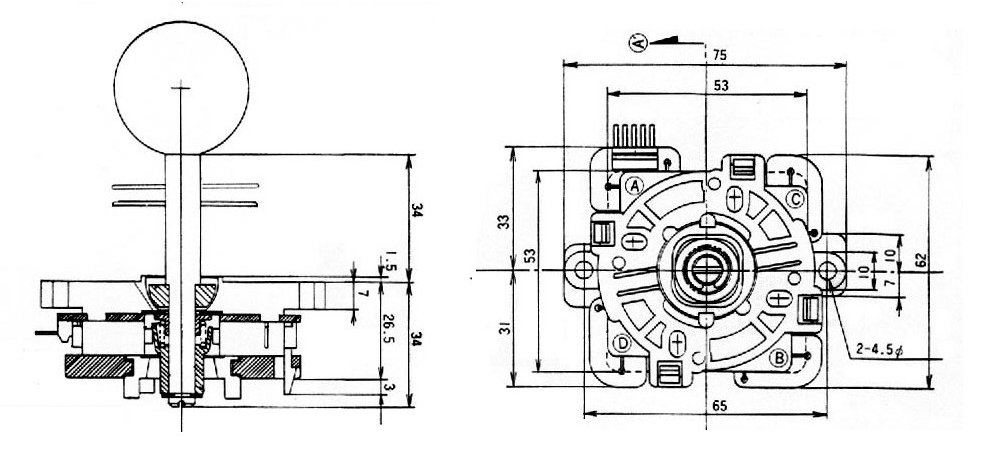
\includegraphics[scale=0.4]{joystick}
\centering
\caption{Sanwa JLF-TP-8YT (measurements in mm)}
\label{fig:joystick}
\end{figure}
\\The joystick’s components are:\\
\textbf{Top}: The handle.\\
\textbf{Stick}: The rod in the joystick.\\
\textbf{Disk}: A plastic disk that facilitates hand movement hand movement. This cover also serves an esthetic purpose of covering the hole housing the joystick.\\
\textbf{Mounting Plate}: The plate of the joystick used to connect the joystick to the control panel.\\
\textbf{Pivot}: The part that permits the movement of the rod.\\
\textbf{Spring}: The mechanism most joysticks use for automatically resetting the stick to the neutral position. The wider the spring is stretched, the greater the resistance to movement that is exerted by the joystick.\\
\textbf{Microswitches}: The switches on which the stick will exert pressure. There are four of them on this joystick.\\
\textbf{Restrictor Gate}: The restrictor is a plastic piece used to limit stick movements.\\
\textbf{Actuators}: It’s a thickness situated in the final part of the stick. It should increase the precision  of the stick and more accurate pression on the microswitches.\\
\textbf{E-ring}: The spring compressor. It helps the stick to return to its neutral position. It’s called like this because it’s form is very similar to an “E”.\\
\newpage
\subsection{ Plancia ed Encoding dei tasti}
La scheda di encoding usata è \textit{I-PAC 2 FS32 KEYBOARD ENCODER}. Una scheda di encoding serve a trasformare segnali elettrici in segnali di input comprensibili ad un personal computer. In pratica è come se ogni microswitch fosse il pulsante di una normale tastiera.\\La \textit{I-PAC 2} riesce a gestire fino a 32 segnali di input (trackball esclusa), più che sufficienti dato che per il progetto ne sono bastate 26. Il DataSheet seguente (Figura~\ref{fig:ke}) riporta tutte le caratteristiche del componente.\\
\begin{figure}[!ht]
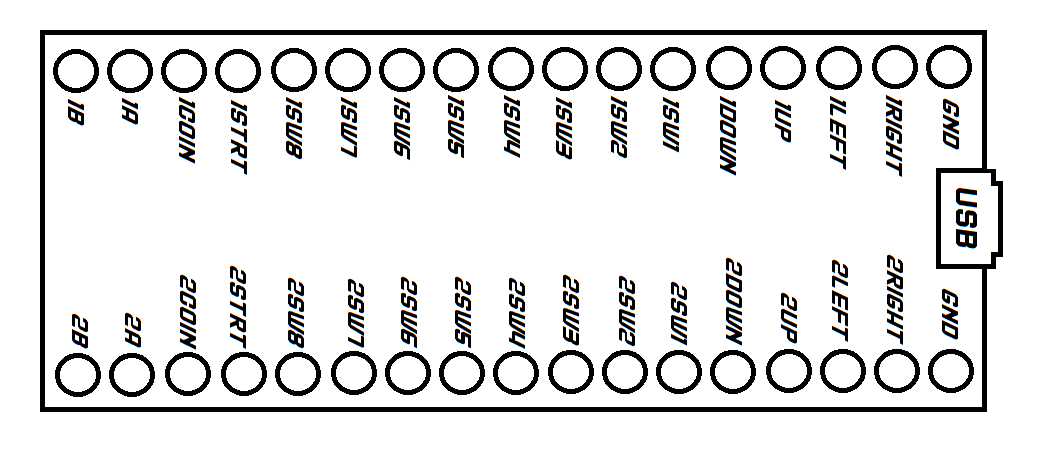
\includegraphics[scale=0.4]{card}
\centering
\caption{DataSheet I-PAC 2 FS32 Keyboard Encoder}
\label{fig:ke}
\end{figure}
\\GND è la massa in comune per tutti i microswitch.Gli otto ingressi denominati Right Left Up e Down per entrambi i giocatori sono i pin per i movimenti delle leve. Gli ingressi che vanno da SW1 a SW8 per entrambi i giocatori sono invece i pin dei bottoni. SW7 ed SW8 Non sono utilizzati perchè i pulsanti sulla plancia sono solo sei per giocatore. I due STRT sono i pin dei pulsanti di Start mentre COIN sono quelli di inserimento crediti.\\Come si può notare dall’immagine, la scheda di encoding si collega al computer tramite un cavetto usb mini. Il sistema riconosce il dispositivo di input come “dispositivo di gioco”, ed effettivamente il suo funzionamento non è affatto diverso da quello di un joypad. Tramite il software messo a disposizione dall'azienda che ha rilasciato la scheda, è possibile configurare tutti i tasti e le leve. Questo è un passaggio fondamentale in quanto servirá successivamente durante la fase di bind dei tasti per ogni emulatore.\\La disposizione dei bottoni e dei Joystick sulla plancia è riportata qui sotto (Figura~\ref{fig:plancia}):\\
\begin{figure}[!ht]
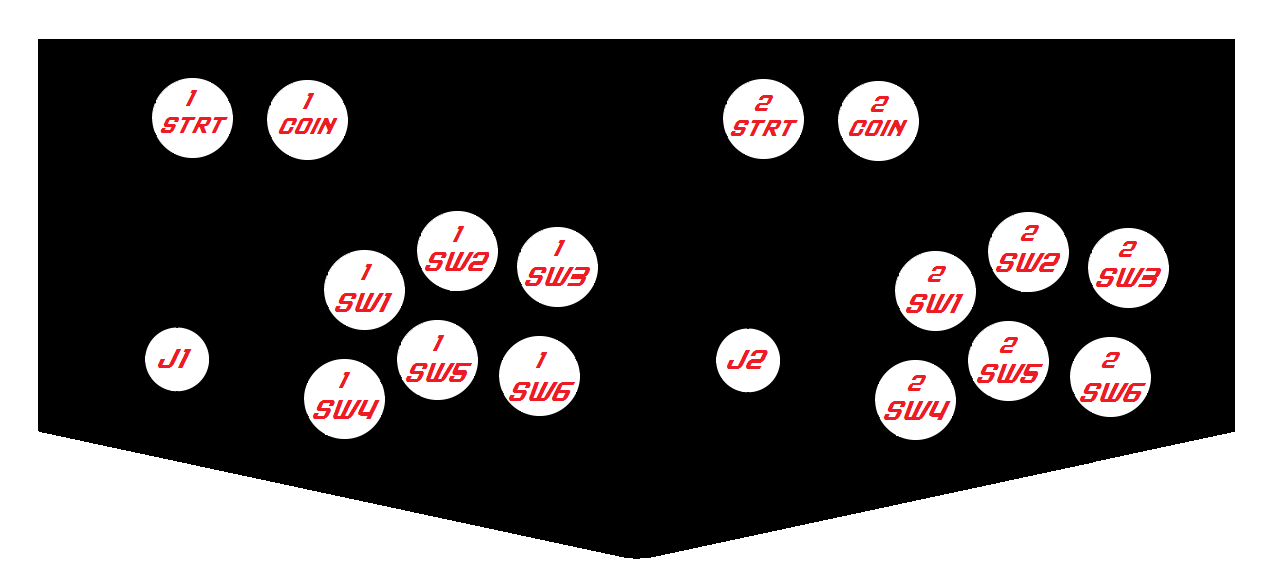
\includegraphics[scale=0.3]{plancia}
\centering
\caption{Disposizione dei tasti sulla Plancia }
\label{fig:plancia}
\end{figure}
\newpage
\subsection{Gestione elettricità}
All’interno del cabinato non c’è altro che un normalissimo Personal Computer che segue l'architettura di Von Neumann e in quanto tale ha bisogno di un alimentatore per funzionare correttamente. Lo standard usato per gli alimentatori è ATX, inizialmente ideato da Intel e ora standard mondiale di ogni PC.\\
I componenti da alimentare quindi sono:\\
\begin{itemize}
\item L’alimentatore del PC
\item Il monitor
\item Gli altoparlanti
\item I led dei pulsanti sulla plancia
\item La striscia di led estetici
\end{itemize}
All’interno del cabinet è stata inserita una multipresa che viene alimentata solo se l’interruttore generale posizionato nella parte superiore del mobile (sopra il monitor) è acceso.
L'alimentazione dello schermo, delle casse, dei led estetici e dell'alimentatore non costituiscono un problema, in quanto dispongono giá di un cavo proprietario che fornisce loro corrente. Il problema sorge solo per i pulsanti sulla plancia, dato che devono essere alimentati con 12V di tensione ma non si dispone di nessun tipo di cavo in dotazione per il collegamento all’elettricità. È importante notare che l’alimentazione serve solo per far funzionare i led e non i Microswitch che invece vengono alimentati tramite una porta usb del PC (Figura~\ref{fig:uio}) e quindi indirettamente dall’alimentatore. Ci sono due strade per fornire il voltaggio ai pulsanti: si può procurare tramite un cavo apposito (creabile) da collegare anch’esso alla multipresa, o si possono ottenere dall’alimentatore. Un alimentatore ATX infatti consente di estrapolare alcuni dei voltaggi più famosi e utili, che permettono di eseguire la maggior parte di test elettrici. Le tensioni che possono essere emesse sono tre: 3V, 5V, 12V  e quindi anche le loro controparti negative tramite i cavi, distinguibili per colore. Il cavo dei 3V è arancione, quello dei 5V è rosso, quello da 12V è giallo e la massa è qualsiasi cavetto nero. Notiamo subito che i 12V sono effettivamente estrapolabili direttamente dall’alimentatore del PC. Tutti i bulb holder vanno quindi collegati in parallelo, con una massa comune. Ogni polo positivo di ciascuno bulb holder è stato quindi collegato con la carica positiva di un altro, fino ad arrivare ad una situazione in cui tutti i bulb holder hanno un solo collegamento con un altro medesimo. Un solo bulb holder poi deve essere collegato al cavo giallo dei 12V dell’alimentazione. La stessa operazione è stata eseguita per i poli negativi, ma usando il cavo nero della massa. La connessione in parallelo è molto più pratica di quella in serie in questo caso, perchè se cede la connessione con un pulsante, gli altri continuano a funzionare indipendentemente dalla rottura. Se invece ci fosse un guasto in una connessione in serie, tutti i diodi a valle della rottura smetterebbero di alimentarsi automaticamente. Inoltre una connessione in serie renderebbe squilibrata l’intensità dei led. Il primo led della serie avrebbe una tonalità molto più decisa dell’ultimo, che anzi, forse sarebbe addirittura spento.\\È importante sottolineare che la massa dell’alimentatore e quella della scheda di encoding non devono assolutamente essere confuse, in quanto sono masse diverse di due sistemi completamente indipendenti l’uno dall’altro.
\begin{figure}[!ht]
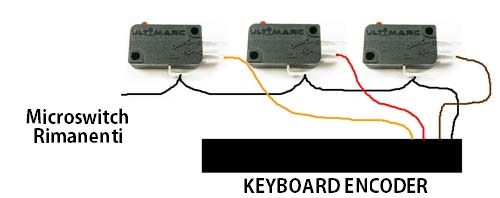
\includegraphics[scale=2.3]{uio_wiring}
\centering
\caption{Collegamento dei Microswith alla Keyboard Encoder}
\label{fig:uio}
\end{figure}
\newpage
\section{Software}
La scelta del sistema operativo e dei software da utilizzare è molto importante. È fondamentale ricordare che il computer deve essere di tipo special purpose, cioè dedicato ad una sola applicazione specifica. Se un normale pc (general purpose) è estremamente versatile e può eseguire diversi tipi di applicazioni, il computer nel mobile deve limitarsi a fungere da emulatore. Esistono migliaia di emulatori completamente gratuiti in giro per il web, per ogni OS.
\subsection{Sistema Operativo}
La scelta del sistema operativo non è stata affatto scontata. Sarebbe stato possibile installare Windows XP con il relativo emulatore proprietario, ma la scelta in questo caso si è incentrata soprattutto sull’emulatore. L’emulatore che è stato usato, che verrà approfondito nel prossimo capitolo, poteva essere installato solo su Linux o su un Raspberry Pi. I sistemi operativi consigliati per la sua installazione sono Ubuntu 16.04 o una qualsiasi distro basata su Debian. Proprio per questo, è stato installato Linux Mint  (Figura~\ref{fig:mint}), una distribuzione GNU/Linux per personal computer, nota per la sua facilità d'uso e per la sua semplicità di installazione. È basata su Ubuntu (a sua volta basata su Debian) e usa sia repository proprie sia di Ubuntu.\\
\begin{figure}[!ht]

\includegraphics[scale=0.2]{mint}
\centering
\caption{Logo di Linux Mint}
\label{fig:mint}
\end{figure}
\\È una delle distro più scaricate ed usate a causa della sua facilità di utilizzo.\\Essendo basata su Debian e Ubuntu, garantisce circa 30,000 package.\\Linux Mint richiede veramente poca manutenzione e nessuna particolare precauzioni contro virus e spyware.\\La scelta di Linux è stata anche influenzata dalla poca potenza hardware disponibile. Windows contiene numerosi processi in background capaci di rallentare l’emulazione di un gioco, già di per sé faticosa. È inoltre risaputo che Windows non è il sistema operativo più vantaggioso quando si tratta di compiti univoci e specifici, in quanto contiene dei componenti pesanti adatti ad una macchina di tipo general purpose. Come verrà però ribadito nella sezione degli sviluppi futuri, un’installazione in una partizione secondaria di un sistema Windows potrebbe essere utile per alcuni giochi disponibili soltanto per quella piattaforma specifica.
\subsection{RetroPie}
Uno degli emulatori più famosi è RetroPie (Figura~\ref{fig:rpie}). RetroPie è una vera e propria evoluzione di un altro famosissimo emulatore chiamato emulationstation. Il progetto open source è presente su \textit{GitHub}. Essendo stato scritto in \gls{c}, il software finale risulta molto leggero e richiede pochissima capacità di calcolo. Perfino un Raspberry Pi è in grado di far funzionare senza problema il programma.\\Retropie è un progetto front-end che richiede un numero limitato di configurazioni iniziali e che fornisce invece agli utenti più esperti notevoli possibilità di customizzazione.\\Un’altro componente sfruttato è \textit{RetroArch}, ovvero l’API sviluppata da \textit{Libretro} che standardizza i controlli e aggiunge molteplici feature migliorando l’esperienza di gioco. La compatibilità di molti giochi è possibile proprio grazie al duro lavoro del team di sviluppo \textit{Libretro}. Retroarch fornisce servizi come il netplay o i sistemi di achievement. Per quanto riguarda il lato grafico invece, permette di modificare gli shader in qualsiasi modo, ottenendo combinazioni infinite e ogni volta nuove ed originali. Inoltre permette la registrazione video e addirittura lo streaming dal vivo su \textit{Youtube} e \textit{Twitch}. È anche possibile connettersi ad internet e trasferire rom da un dispositivo di archiviazione o da computer, a patto che sia sulla stessa rete.\\
\begin{figure}[!ht]

\includegraphics[scale=0.17]{rpielogo}
\centering
\caption{Logo di RetroPie}
\label{fig:rpie}
\end{figure}
\\Di base, sono già installati circa una trentina di emulatori ma sono supportati più di 50 sistemi diversi. Retropie può essere installato su Raspbian, Raspberry Pi, Debian e Ubuntu, ragion per cui sul PC non può che essere installato un sistema Linux. Gli sviluppatori dell’emulatore consigliano l’installazione su Debian, su una relativa distro come Linux Mint 17 e 18 o su Ubuntu 16.04 LTS.\\L’installazione del software è molto semplice e pratica. Essendo presente su \textit{GitHub}, è possibile eseguire tutta l’operazione tramite il terminale di sistema. È innanzitutto opportuno installare i package necessari, scaricare il setup script con il comando \textit{git clone} e infine avviare lo script presente all’interno del progetto. L’installazione avviene come in un normale Setup Wizard. Per la configurazione la procedura è più o meno simile. Sempre da terminale, a installazione eseguita, è sufficiente scrivere emulationstation per aprire il menù delle impostazioni. In questo menù si possono trovare, oltre a configurazioni sulla risoluzione e i comandi dei giochi, anche impostazioni utili e importanti come l’autostart dell’emulatore all’avvio del PC. In realtà basterà configurare i controlli una sola volta, e questo avverrà al primo avvio di Retropie. Se infatti verrà rilevato un dispositivo di input, apparirà la richiesta di configurazione dei tasti. Sarà poi Retroarch a scegliere automaticamente quali tasti usare basandosi sull’emulatore che verrà utilizzato. È anche possibile configurare gli hotkey, cioè le combinazioni di tasti per determinate funzioni (come l’uscita dal gioco). Grazie alla funzione Scraper dai menù dell’emulatore è possibile, se connessi ad internet, scaricare da alcuni server le copertine o immagini significative rappresentanti il gioco selezionato.\\Alcuni emulatori presenti in Retropie hanno bisogno di un BIOS per funzionare correttamente e per evitare situazioni di crash. I nomi file dei BIOS non vanno assolutamente rinominati e le lettere maiuscole vanno rispettate. Tutti i BIOS sono già all’interno del progetto GitHub di Retropie per questioni legali, l’unica cosa da fare è spostarli nella cartella /home/pi/RetroPie/BIOS/.\\Uno dei BIOS più utilizzati è quello delle rom MAME, per esempio neogeo.zip è indispensabile per avviare i giochi \gls{snk} e NeoGeo, i quali appunto utilizzano emulatori MAME.\\Il file neogeo.zip è particolare. A differenza degli altri BIOS va inserito nella stessa cartella delle rom dell’emulatore MAME usato.\\Sul sito ufficiale di Retropie in ogni caso, è a disposizione di tutti una tabella con tutti i nomi dei BIOS e la posizione corretta in cui metterli. Una ROM può presentarsi in svariati formati ed estensione dipendentemente dall’emulatore per cui sono supportati.
